\documentclass[border=6pt]{standalone}
\usepackage{tikz}
\usetikzlibrary{arrows.meta,calc}
\begin{document}
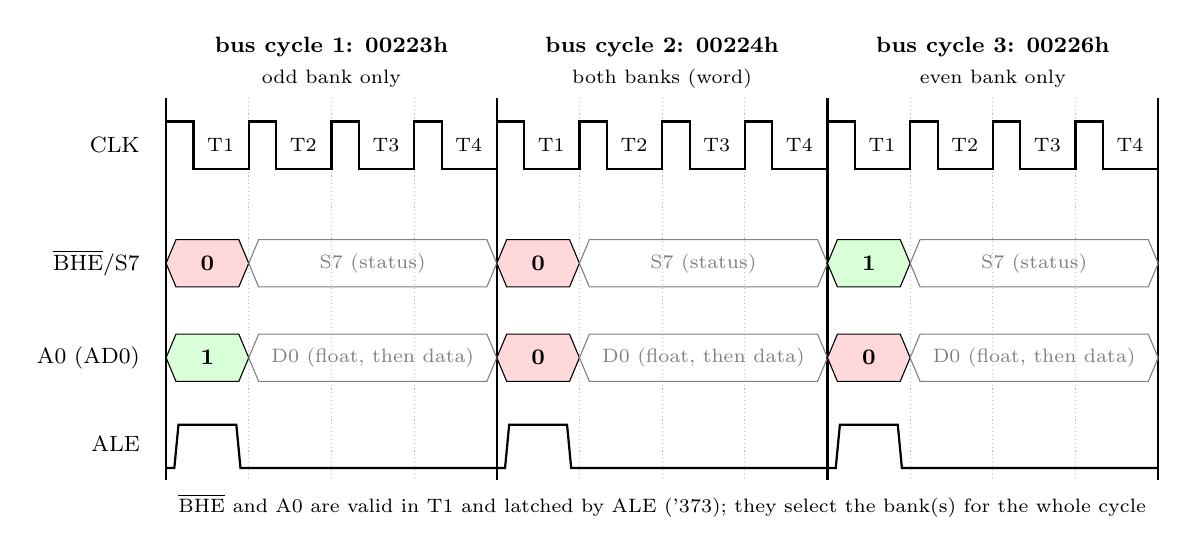
\begin{tikzpicture}[>=Stealth,font=\small,x=1.05cm,y=1cm]
% 12 T-states, one unit each; 3 bus cycles of T1-T4
\def\s{0.12}% slant of a signal transition
% cycle headers
\foreach \c/\a/\b in {0/00223h/odd bank only,1/00224h/both banks (word),2/00226h/even bank only} {
  \draw[thick] (4*\c,0.9) -- (4*\c,-3.95);
  \node[font=\footnotesize\bfseries] at (4*\c+2,1.55) {bus cycle \the\numexpr\c+1\relax: \a};
  \node[font=\scriptsize] at (4*\c+2,1.15) {\b};
}
\draw[thick] (12,0.9) -- (12,-3.95);
\foreach \x in {1,2,3,5,6,7,9,10,11} \draw[gray!50,densely dotted] (\x,0.9) -- (\x,-3.95);
% CLK: 8086 clock, 33% duty (high for the first third of each T state)
\node[anchor=east,font=\footnotesize] at (-0.2,0.3) {CLK};
\draw[thick] (0,0) \foreach \t in {0,...,11} { -- (\t,0) -- (\t,0.6) -- (\t+0.333,0.6) -- (\t+0.333,0) } -- (12,0);
\foreach \t in {0,...,11} {
  \pgfmathtruncatemacro{\k}{mod(\t,4)+1}
  \node[font=\scriptsize] at (\t+0.66,0.3) {T\k};
}
% helper: bus-style row: valid value during T1, then other use
% BHE'/S7 row
\node[anchor=east,font=\footnotesize,align=right] at (-0.2,-1.2) {$\overline{\mathrm{BHE}}$/S7};
\foreach \c/\v/\col in {0/0/red!15,1/0/red!15,2/1/green!15} {
  \fill[\col] (4*\c+\s,-0.9) -- (4*\c+1-\s,-0.9) -- (4*\c+1,-1.2) -- (4*\c+1-\s,-1.5) -- (4*\c+\s,-1.5) -- (4*\c,-1.2) -- cycle;
  \draw (4*\c,-1.2) -- (4*\c+\s,-0.9) -- (4*\c+1-\s,-0.9) -- (4*\c+1,-1.2) -- (4*\c+1-\s,-1.5) -- (4*\c+\s,-1.5) -- cycle;
  \node[font=\footnotesize\bfseries] at (4*\c+0.5,-1.2) {\v};
  \draw[gray] (4*\c+1,-1.2) -- (4*\c+1+\s,-0.9) -- (4*\c+4-\s,-0.9) -- (4*\c+4,-1.2) -- (4*\c+4-\s,-1.5) -- (4*\c+1+\s,-1.5) -- cycle;
  \node[font=\scriptsize,gray] at (4*\c+2.5,-1.2) {S7 (status)};
}
% A0 / AD0 row
\node[anchor=east,font=\footnotesize,align=right] at (-0.2,-2.4) {A0 (AD0)};
\foreach \c/\v/\col in {0/1/green!15,1/0/red!15,2/0/red!15} {
  \fill[\col] (4*\c+\s,-2.1) -- (4*\c+1-\s,-2.1) -- (4*\c+1,-2.4) -- (4*\c+1-\s,-2.7) -- (4*\c+\s,-2.7) -- (4*\c,-2.4) -- cycle;
  \draw (4*\c,-2.4) -- (4*\c+\s,-2.1) -- (4*\c+1-\s,-2.1) -- (4*\c+1,-2.4) -- (4*\c+1-\s,-2.7) -- (4*\c+\s,-2.7) -- cycle;
  \node[font=\footnotesize\bfseries] at (4*\c+0.5,-2.4) {\v};
  \draw[gray] (4*\c+1,-2.4) -- (4*\c+1+\s,-2.1) -- (4*\c+4-\s,-2.1) -- (4*\c+4,-2.4) -- (4*\c+4-\s,-2.7) -- (4*\c+1+\s,-2.7) -- cycle;
  \node[font=\scriptsize,gray] at (4*\c+2.5,-2.4) {D0 (float, then data)};
}
% ALE
\node[anchor=east,font=\footnotesize] at (-0.2,-3.5) {ALE};
\draw[thick] (0,-3.8) \foreach \c in {0,1,2} { -- (4*\c+0.1,-3.8) -- (4*\c+0.15,-3.25) -- (4*\c+0.85,-3.25) -- (4*\c+0.9,-3.8) } -- (12,-3.8);
\node[font=\scriptsize,align=center,anchor=north] at (6,-4.0) {$\overline{\mathrm{BHE}}$ and A0 are valid in T1 and latched by ALE ('373); they select the bank(s) for the whole cycle};
\end{tikzpicture}
\end{document}
